\documentclass{beamer}
\usepackage{../common_slides}


\title{Part-of-Speech Tagging \\ + \\ Neural Networks 3 }  }
\date{}
\author{CS 287}
\begin{document}


\begin{frame}
  \titlepage
\end{frame}


\begin{frame}{Review: Neural Networks}
  One-layer multi-layer perceptron architecture,

  \[NN_{MLP1}(\boldx) =  g(\boldx\boldW^1 + \boldb^1)W^2 + \boldb^2\]
  \begin{itemize}
  \item $\boldx\boldW + \boldb$; \textit{perceptron}
  \item $\boldx$ is the dense representation in $\reals^{1 \times \din}$
  \item $\boldW^1 \in \reals^{\din \times \dhid}, \boldb^1 \in \reals^{1 \times \dhid}$; first affine transformation
  \item $\boldW^2 \in \reals^{\dhid \times \dout}, \boldb^2 \in \reals^{1 \times \dout}$; second affine transformation
  \item $g:\reals^{\dhid \times \dhid}$ is an \textit{activation non-linearity} (often pointwise)
  \item $g(\boldx\boldW^1 + \boldb^1)$ is the \textit{hidden layer}
  \end{itemize}
\end{frame}

\begin{frame}{Review: Non-Linearities Tanh}
  Hyperbolic Tangeant:
  \begin{figure}
    \centering
    \[\tanh(t) = \frac{\exp(t) - \exp(-t)}{\exp(t) + \exp(-t)}  \]
    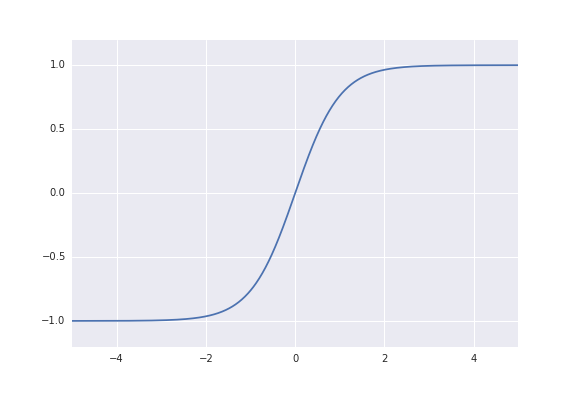
\includegraphics[width=5cm]{../notebooks/tanh}
    \includegraphics[width=5cm]{../notebooks/tanhgrad}
  \end{figure}
  \begin{itemize}
  \item Intuition: Similar to sigmoid, but range between 0 and -1.
  \end{itemize}
\end{frame}

\begin{frame}{Review: Backpropagation}
  \begin{center}

  \begin{tikzpicture}
    \node(x){$f_{i}(\ldots f_{1}(\boldx^0)) $};
    \node(t)[below right= of x, draw]{$f_{i+1}(*;\btheta_{i+1})$};

    \node(fx)[above right=of t]{$f_{i+1}(f_{i}(\ldots f_{1}(\boldx^0)))$};
    \node(gradin)[below left =of t]{$\displaystyle \frac{\partial L}{\partial f_i(\ldots f_1(\boldx^0))  } $};
    \node(gradout)[below right= of t]{$\displaystyle  \frac{\partial L}{\partial f_{i+1}(\ldots f_1(\boldx^0))  }  $};
    \node(gradweight)[below = of t, yshift=1cm]{$\displaystyle  \frac{\partial L}{\partial \btheta_{i+1}  }$};
    \path[draw, ->] (x) -> (t);
    \path[draw, ->] (t) -> (fx);
    \path[draw, ->] (t) -> (gradin);
    \path[draw, ->]  (gradout) -> (t);
  \end{tikzpicture}
  \end{center}
\end{frame}


\begin{frame}{Quiz}
  One common class of operation in deep learning models is known as
  \textit{pooling}. Informally a pooling layer consists of aggregation
  unit, typically unparameterized, that reduce the input to a smaller
  size.
  \air 

  Consider three pooling functions of the form $f: \reals^n \mapsto \reals$, 
  \begin{enumerate}
  \item $ f(\boldx) = \max_{i} x_i $
  \item $ f(\boldx) = \min_{i} x_i $
  \item $ f(\boldx) = \sum_i x_i / |\boldx| $
  \end{enumerate}
  \air

  What action do each of these functions have? What are their gradients? 
  How would you implement backpropagation for these units? 
\end{frame}

\begin{frame}{Quiz}
  \begin{itemize}
  \item \textbf{Max pooling}:  $f(\boldx) = \max_{i} x_i$
    
    \begin{itemize}
    \item Keeps only the most activated input
    \item Fprop is simple; however must store $\argmax$ (``switch'')
    \item Bprop gradient is zero except for switch, which gets gradoutput
    \end{itemize}
    \pause 

  \item \textbf{Min pooling}: $ f(\boldx) = \min_{i} x_i $
    \begin{itemize}
    \item Keeps only the least activated input
    \item Fprop is simple; however must store $\argmin$ (``switch'')
    \item Bprop gradient is zero except for switch, which gets gradoutput
    \end{itemize}
    \pause 
    
  \item \textbf{Avg pooling}: $ f(\boldx) = \sum_i x_i / |\boldx| $
    \begin{itemize}
    \item Keeps the average activation input
    \item Fprop is simply mean. 
    \item Gradoutput is averaged and passed to all inputs.
    \end{itemize}
  \end{itemize}
\end{frame}

\begin{frame}{What to do about words?}
  \begin{center}
    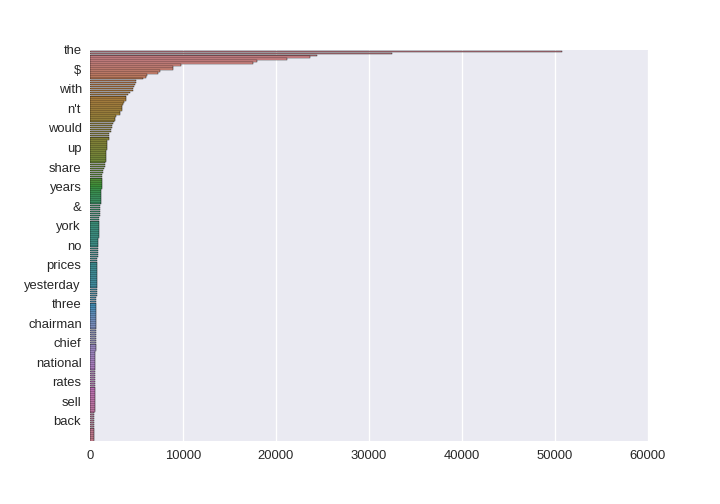
\includegraphics[width=0.8\textwidth]{../notebooks/zipf}         
  \end{center}
\end{frame}

\begin{frame}{Bilinear Model}
  Bilinear model,
  \[\hat{\boldy} = f((\boldx^0 \boldW^0)\boldW^1 + \boldb)\]
  \begin{itemize}
  \item $\boldx^0 \in \reals^{1 \times d_0}$ start with one-hot.
  \item $\boldW^0 \in \reals^{d_0 \times \din}$, $d_0 = |\mcF|$
  \item $\boldW^1 \in \reals^{\din \times \dout}, \boldb \in \reals^{1 \times \dout}$; model parameters
  \end{itemize}
  \air
  Notes:
  \begin{itemize}
  \item Bilinear parameter interaction.
  \item $d_0 >> \din$, e.g. $d_0 = 10000, \din = 50$
  \end{itemize}
\end{frame}

\begin{frame}{Representations}
  \begin{itemize}
  \item We would like shared representations of words
    \air 

  \item However, PTB only 1M words, relatively small

    \air
  \item Collobert et al. (2008, 2011) propose semi-supervised method.

    \air
  \item [Close connection to Bengio et al (2003) (next topic)]
  \end{itemize}
\end{frame}

\begin{frame}{Semi-Supervised Training }
  \textbf{Idea:} Train representations separately on more data

  \begin{enumerate}
  \item Pretrain word embeddings $\boldW^0$ first.
  \item Substitute them in as first NN layer
  \item (Optional) Fine-tune embeddings for final task
  \end{enumerate}
\end{frame}

\begin{frame}{New Corpora}
  To learn rare word embeddings, need many more tokens,

  \begin{itemize}
  \item English Wikipedia (631 million words tokens)
    \air 
  \item Reuters Corpus (221 million word tokens)
    \air 
  \item Total vocabulary size: 130,000 word types 
  \end{itemize}

  But this data has no labels...
\end{frame}

\begin{frame}{C\&W Embeddings}
  \begin{itemize}
  \item All text in Wikipedia in some sense coherent. 
    \air
  \item Good embeddings should be able to help distinguish coherent text from nonsense
    \air 

  \item We can train on this task.
  \end{itemize}
\end{frame}


\begin{frame}{C\&W Setup}
  Let $\mcV$ be the vocabulary of English and let $s$ 
  score any window of size $\dwin$, if we see the phrase

  \begin{itemize}
  \item [ the dog walks to the ]
  \end{itemize}

  It should score higher by $s$ than 

  \begin{itemize}
  \item [ the dog \alert{house} to the ]
  \item [ the dog \alert{cats} to the ]
  \item [ the dog \alert{skips} to the ]
  \item ...
  \end{itemize}
\end{frame}

\begin{frame}{C\&W Setup}
  Can estimate $s$ as a windowed neural network.

  \[ s(w_1, \ldots, w_{\dwin}) = \mathrm{hardtanh}(\boldx \boldW^1 + \boldb^1) \boldW^2 + \boldb \] 
  with 
  \[ \boldx = [v(w_1)\  v(w_2) \  \ldots \  v(w_{\dwin})]  \]

  \begin{itemize}
  \item $\din = \dwin \times 50$, $\dhid = 100$, $\dwin=11$, \alert{$\dout = 1$}!  
  \end{itemize}

  Example: Function $s$
  \[ \boldx = [v(w_3)\  v(w_4) \  v(w_5) \ v(w_6) \ v(w_7)]  \]

  \[\renewcommand\matscale{.6}
  \matbox{1.5}{4}{\din /\dwin}{} \matbox{1.5}{4}{\din /\dwin}{} \matbox{1.5}{4}{\din /\dwin}{\boldx} \matbox{1.5}{4}{\din /\dwin}{} \matbox{1.5}{4}{\din /\dwin}{}\]
\end{frame}

\begin{frame}{Training?}
  \begin{itemize}
  \item Different setup than previous experiments.

    \air 
  \item 
  \end{itemize}
end{frame}


\begin{frame}{Ranking Loss}
  Given only example $\{ \boldx_1, \ldots, \boldx_n \}$ and for 
  each example have set $\mcD(\boldx)$ of alternatives. 
  
  \[ \mathcal{L} = \sum_i \sum_{\boldx' \in \mcD(\boldx)} L_{ranking}(s(\boldx_i), s(\boldx') \] 

  \[ L_{ranking}(y, \hat{y}) = \max\{0, 1 - (y - \hat{y}) \}   \] 

  \textbf{Example:} C\&W ranking

  $\boldx =$ [the dog walks to the] 

  $\mcD(\boldx) = \{$ [the dog skips to the], [the dog in to the], \ldots $\}$

  \begin{itemize}
  \item [Torch \texttt{nn.RankingCriterion}]
    \air 
  \item Note: slightly different setup, both $s(\boldx_i)$ and $s(\boldx')$ receive gradient.
  \end{itemize}
\end{frame}

\begin{frame}
  \begin{itemize}
  \item Vocabulary size $|\mcD(\boldx)| > 100,000$
    \air 
    
  \item Training time for 4 weeks
    \air 

  \item (guy who invented torch)
  \end{itemize}
\end{frame}

\begin{frame}{WSABIE}
  \textbf{Observation:} in many contexts  
  \[ L_{ranking}(y, \hat{y)} = \max\{0, 1 - (y - \hat{y}) \} = 0 \]

  \air 
k
  But for difficult contexts, may be easy to find 

  \[ L_{ranking}(y, \hat{y)} = \max\{0, 1 - (y - \hat{y}) \} \neq 0 \]
  
  We can therefore sample from $\mcD(\boldx)$ to find an update.
    
\end{frame}

\begin{frame}
  \begin{center}
    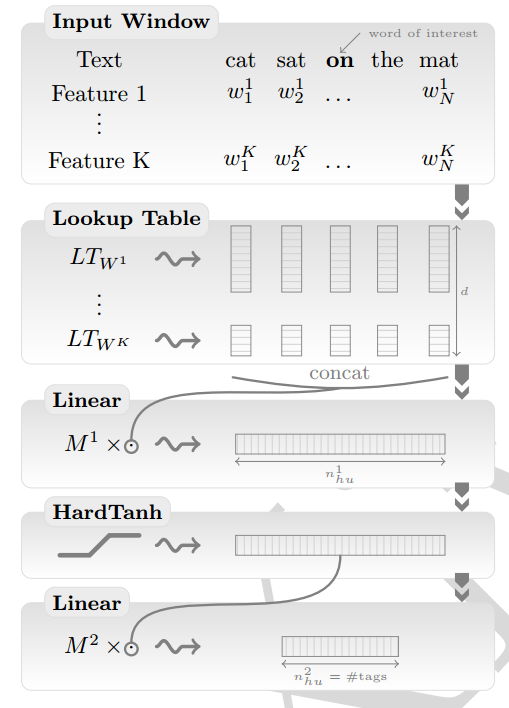
\includegraphics[width=5cm]{cwfull}
  \end{center}
  \begin{enumerate}
  \item Use dense representations instead of sparse
  \item Use windowed area instead of sequence models
  \item Use neural networks to model windowed interactions
  \item Use semi-supervised learning to pretrain representations.
  \end{enumerate}
\end{frame}

\begin{frame}{Other Embedding Method: word2vec}
  \begin{itemize}
  \item Instead of MLP uses Bilinear model (``linear'' in paper)
    \air 

  \item Instead of ranking model, directly predict word (cross-entropy)
    \air 

  \item Two different models 
    \begin{enumerate}
    \item Skipgram
    \item Continuous Bag-of-Words (CBOW)
    \end{enumerate}

  \item Various other ideas. 
    
  \end{itemize}
\end{frame}

\section{word2vec}

\begin{frame}{word2vec}
  
\end{frame}

\begin{frame}{Continuous Bag-of-Words (CBOW) }
  \begin{itemize}
  \item Bag-of-words bilinear model, after embedding
  \item Attempt to predict the middle word
  \end{itemize}

  Example: CBOW
  \[ \boldx = v(w_3) +  v(w_4) +   v(w_6) + v(w_7)/$\dwin-1$   \]
  \[ \boldy = \delta(w_5) \]

  \[\renewcommand\matscale{.6}
  \matbox{1.5}{4}{\din }{} + \matbox{1.5}{4}{\din }{} + \matbox{1.5}{4}{\din }{\boldx} + \matbox{1.5}{4}{\din }{} + \matbox{1.5}{4}{\din }{}\]  

  $\boldW^1$ is no longer partitioned by row  
\end{frame}


\begin{frame}{Skipgram}
  \begin{itemize}
  \item Also a bilinear model, after embedding
  \item Attempt to predict outer word from middle 
  \end{itemize}

  Example: CBOW
  \[ \boldx = v(w_5)$   \]
  \[ \boldy = \delta(c)\ \mathrm{\ where\ } c \in \{w_3, w_4,w_6, w_7\}  \]

  \[\renewcommand\matscale{.6}
  \matbox{1.5}{4}{\din }{} + \matbox{1.5}{4}{\din }{} + \matbox{1.5}{4}{\din }{\boldx} + \matbox{1.5}{4}{\din }{} + \matbox{1.5}{4}{\din}{} \]  

  $\boldW^1$ is no longer partitioned by row  
\end{frame}

\begin{frame}{Softmax}
  
\end{frame}

\begin{frame}{Hierarchical Softmax}

  
  
\end{frame}

\begin{frame}{Negative Sampling}
  
\end{frame}

\begin{frame}{Embedding Tasks}
  
\end{frame}

\begin{frame}{Other Elements}
  \begin{itemize}
  \item At each SGD step $\dwin$ is sampled 

  \item Frequent words are used less
  \end{itemize}  
\end{frame}

\section{Comparing Embeddings}

\begin{frame}
  
\end{frame}

\section{Visualizing Embeddings}

\begin{frame}
 
\end{frame}


\begin{frame}
  
\end{frame}


\end{document}

